\documentclass[10pt,a4j,dvipdfmx]{jsarticle}
\usepackage[utf8]{inputenc}
\usepackage[dvipdfmx]{graphicx}
\usepackage[usenames,dvipdfmx]{color}
\usepackage{amsmath}
\usepackage{bm}
\usepackage[left=19.05mm, right=19.05mm, top=25.40mm, bottom=25.40mm]{geometry}
\usepackage{tikz}
\usepackage{circuitikz}
\usepackage{siunitx}
\usepackage{listings}
\usepackage{float}
\usepackage{hyperref}

\lstset{%
  language={C},
  basicstyle={\small},%
  identifierstyle={\small},%
  commentstyle={\small\itshape},%
  keywordstyle={\small\bfseries},%
  ndkeywordstyle={\small},%
  stringstyle={\small\ttfamily},
  frame={tb},
  breaklines=true,
  columns=[l]{fullflexible},%
  numbers=left,%
  xrightmargin=0zw,%
  xleftmargin=3zw,%
  numberstyle={\scriptsize},%
  stepnumber=1,
  numbersep=1zw,%
  lineskip=-0.5ex%
}

\usepackage{fouriernc}
\usepackage[scaled]{helvet}
\usepackage[T1]{fontenc}
\renewcommand{\ttdefault}{fvm}

\let\oldthefootnote\thefootnote
\def\thefootnote{{\color{Magenta}\oldthefootnote}}

\newcommand{\enhance}[1]{{\gtfamily\sffamily#1}}
\makeatletter
\def\@jikkenname{}
\def\@jikkennum{}
\def\@reportname{}
\def\@studentnumber{}
\def\@studentname{}
\def\@studentdepartment{}
\def\@friendnames{}
\def\@groupnumber{}
\newcommand{\jikkenset}[2]{\def\@jikkennum{#1}\def\@jikkenname{#2}}
\newcommand{\studentset}[3]{\def\@studentnumber{#1}\def\@studentname{#2}\def\@studentdepartment{#3}}
\newcommand{\reportnameset}[1]{\def\@reportname{#1}}
\newcommand{\friendname}[1]{\def\@friendnames{#1}}
\newcommand{\groupnumber}[1]{\def\@groupnumber{#1}}
\renewcommand{\maketitle}{
\noindent{\color{RoyalPurple}\hrule height 1pt \hfill}
\vspace{5pt}
\begin{center}
\enhance{{\Large{電気電子情報第一(前期)実験}}}\\[7pt]
\enhance{{\Huge\textbf{\@jikkennum{}. \@jikkenname}}}\\[5pt]
\enhance{{\LARGE{\@reportname}}}\\[15pt]
\@studentnumber\ \ \ \@studentname{}(\@studentdepartment{})\\[1pt]
共同実験者: \@friendnames(第\@groupnumber{}班)\\[1pt]
\today
\end{center}
\vspace{-10pt}
\noindent{\color{RoyalPurple}\hrule height 1pt \hfill}
}
\makeatother
\jikkenset{P1}{電気回路の基礎}
\reportnameset{考察レポート}
\studentset{03-160441}{土屋潤一郎}{工学部 電子情報工学科}
\friendname{井上友貴、田中大幹、坂口達彦}
\groupnumber{28}

\begin{document}
\maketitle

\section{実験の概要}
\begin{description}
 \item[第1日]計測機器の使用習熟およびはんだによる基板実装習熟。RLC直列回路の周波数特性及びステップ応答の計測。
 \item[第2日]RC四端子網回路の周波数特性及びステップ応答の計測。
\end{description}
\section{考察}
\subsection{伝達関数の極・零点を用いた周波数特性の説明}
s領域(平面)での伝達関数$H(s)$を

\begin{equation}
H(s) = H\bullet\frac{(s-s_{z1})(s-s_{z2})(s-s_{z3})...}{(s-s_{p1})(s-s_{p2})(s-s_{p3})...}
\end{equation}

とすると、その極と零点を用いて、振幅特性$|H(s)|$と位相特性$\b{Arg}$$|H(s)|$が以下のように表せる。

\begin{eqnarray}
\left|H\left(s\right)\right| &=&
\left|H\right|
\frac{\prod_{i} d_{zi}\left(s\right)}
{\prod_{i}d_{pi}\left(s\right)}\\
\b{Arg}\left|H\left(s\right)\right| &=& \sum_{i}\theta_{zi}\left(s\right) - \sum_{i}\theta_{pi}\left(s\right) \\
\end{eqnarray}
ただし、$d_{zi}$はi番目の零点とsとの距離、$d_{pi}$はi番目の極とsとの距離、
$\theta_{zi}$はi番目の零点からsへの偏角、$\theta_{pi}$はi番目の極からsへの偏角である。

\subsubsection{RLC直列共振回路}
2端子回路なので、出力を時間に対する電流波形と考えると、
その伝達関数は、

\begin{equation}
H(s) = \frac{I}{V} = Y
\end{equation}

と、アドミタンスに等しい。

今回28班が用いた回路を簡素化し(コイル内部以外の抵抗成分をまとめる)、
コイル素子を等価回路に置き換えると、
図1のようになる。

\begin{figure}[H]
  \centering
  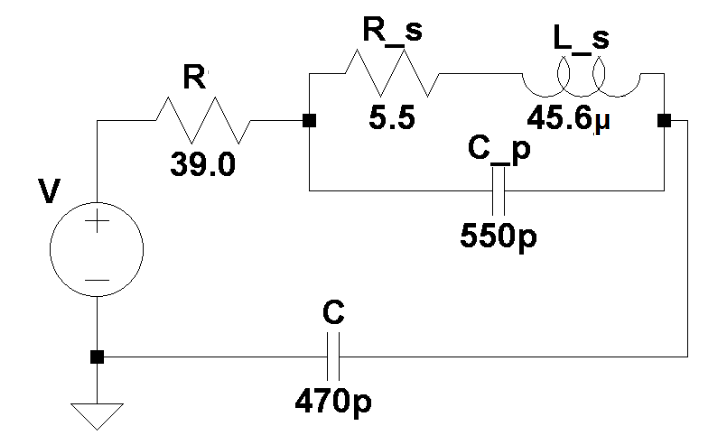
\includegraphics[width=8cm]{RLCkettei.png}
  \caption{測定に用いたRLC直列回路の等価回路}
\end{figure}

この合成アドミタンスを用いて伝達関数を整理すると、

\begin{equation}
H(s) = \frac{1}{R} \bullet \frac{s^{3}+\frac{R_{L}}{L}s^{2}+\frac{1}{C_{L}L}s}
{s^{3}
+\left(\frac{R_{L}}{L}+\frac{1}{C_{L}R}+\frac{1}{CR}\right)s^{2}
+\left(\frac{1}{C_{L}L}+\frac{R_{L}}{C_{L}LR}+\frac{R_{L}}{CLR}\right)s
+\frac{1}{CC_{L}LR}
}
\end{equation}

これに、
\begin{eqnarray}
R &=& 39.0\left[\si{\ohm}\right] \\
R_{s} &=& 5.5\left[\si{\ohm}\right] \\
L_{s} &=& 45.6\bullet10^{-6}\left[\si{\henry}\right] \\
C_{p} &=& 550\bullet10^{-12}\left[\si{\farad}\right] \\
C &=& 470\bullet10^{-12}\left[\si{\farad}\right] \\
\end{eqnarray}
を代入して、極と零点を求める。

伝達関数の極と零点は3つずつで、図2のような配置となる。

値としては、零点が
\begin{eqnarray}
s &=& 0 \\
s &=& -6.05\bullet10^4-6.32\bullet10^6 j \\
s &=& -6.05\bullet10^4+6.32\bullet10^6 j
\end{eqnarray}
で、極が
\begin{eqnarray}
s &=& -9.85\bullet10^7 \\
s &=& -1.54\bullet10^5-4.64\bullet10^6 j \\
s &=& -1.54\bullet10^5+4.64\bullet10^6 j
\end{eqnarray}
である。

\begin{figure}[H]
  \centering
  
\includegraphics[width=5cm]{token.png}
  \caption{RLC直列回路の周波数特性測定に用いた回路のアドミタンスの極と零点}
\end{figure}

さて、周波数はこの虚軸上正の部分を動くから、まず原点では1つの零点との距離が0なので振幅の利得が0なのは当然だが、極・零点ともに3つずつあるのでその振る舞いは一見して共振周波数がわかるほど自明ではない。位相についても同様である。
従って、これらの周波数特性を、(2)式及び(3)式に基づいて数値計算して(実験結果のデータセットとともに)プロットするプログラムを用意した(レポート末付録資料、参考コード1)。その結果のグラフが、図3である。

\begin{figure}[H]
  \centering
  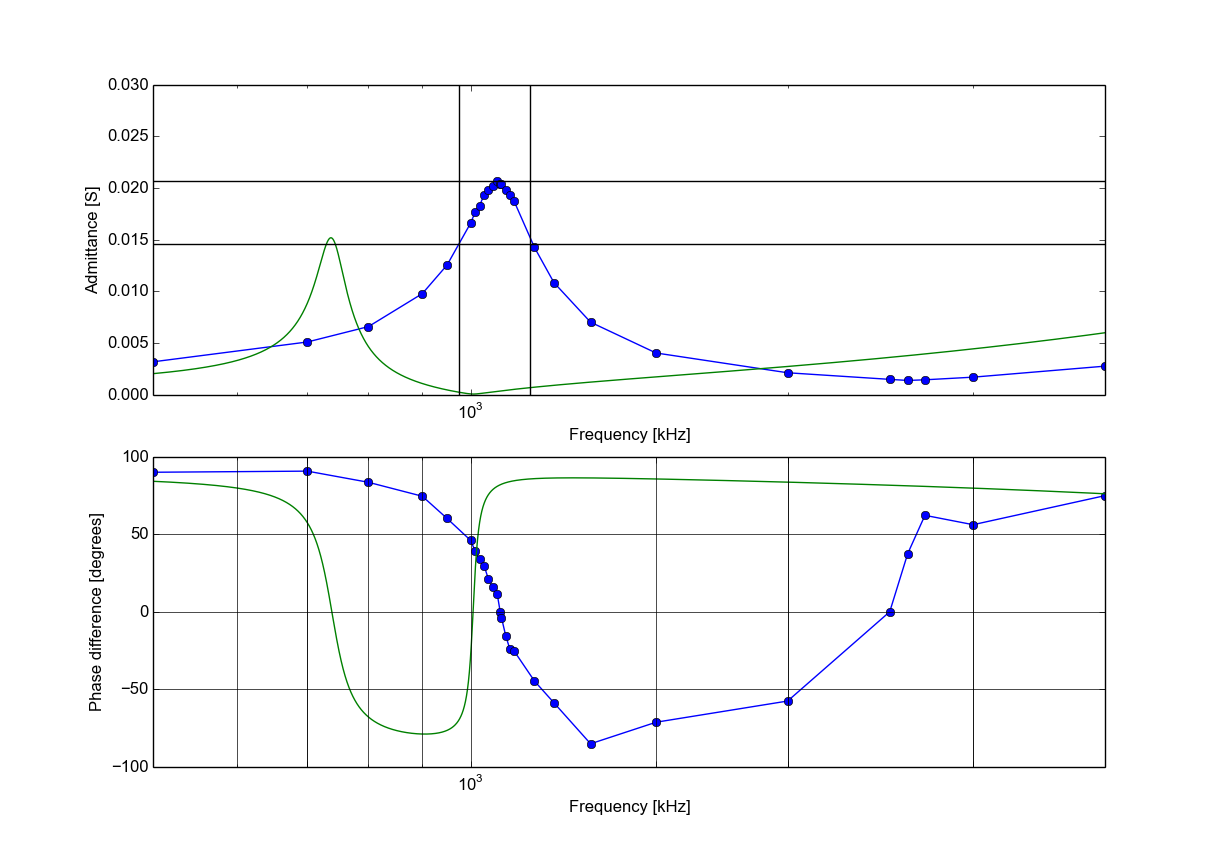
\includegraphics[width=16cm]{P1TF.png}
  \caption{周波数特性の実測値と理論値}
\end{figure}

共振周波数のずれを無視すれば、グラフの概形は一致しているから、伝達関数(6)式の極と零点の位置に依って概形を説明できたと言って良いだろう。
一方、共振周波数の数値については説明できない。原因としては、コイルの並列キャパシタンス成分が挙げられる。
LCRメーターで測定したコイルの並列キャパシタンスは550p[F]であったが、基板にはんだ付けしたことによってこの値が変化した可能性がある。

再び数値計算とプロットを用いる。
レポート末付録資料の参考コード2によって描いた、コイルの並列キャパシタンスが24p[\si{\farad}]だと仮定した場合の振幅特性の理論値曲線が図4である。

\begin{figure}[H]
  \centering
  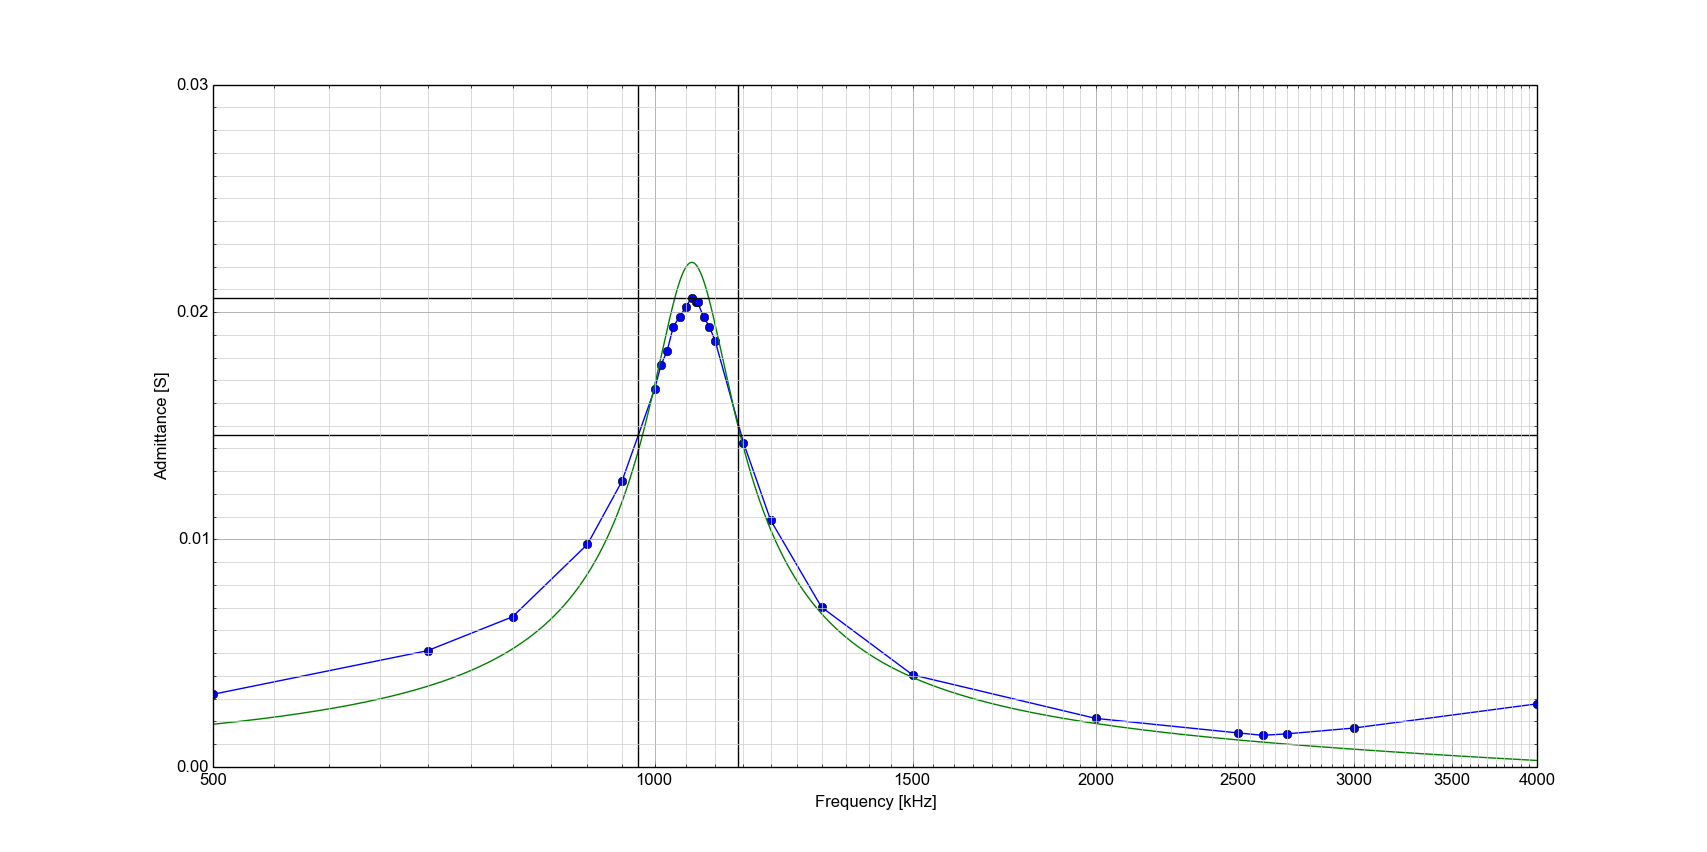
\includegraphics[width=16cm]{P1analyze.png}
  \caption{周波数特性の実測値と理論値($Cp=24*10^{-12}\left[\si{\farad}\right]$の場合)}
\end{figure}

このように、コイルを基板にはんだ付けしたことによってコイルの並列キャパシタンスが低下したと考えられる。
一方、参考資料[2]p17にはインダクタをプリント配線板に実装すると逆に並列キャパシタンスが増加(して自己共振周波数が低下する)旨の記載がある。
従って、LCRメーターでの計測に誤りがあった可能性もある。
いずれにせよ、回路上ではこの並列キャパシタンスの値が小さかったと考えるべきだろう。

一方、アドミタンスのピークやのQ値のずれは、接触抵抗によって説明できる。全体の直列抵抗値が$10^{1}$のオーダーなので、ひと桁オームの接触抵抗でも十分アドミタンスのピークやのQ値が大きく変わりうる。

\subsubsection{LPF}
図5に、測定に用いたRC低域通過フィルタを、素子の値とともに示す。
\begin{figure}[H]
  \centering
  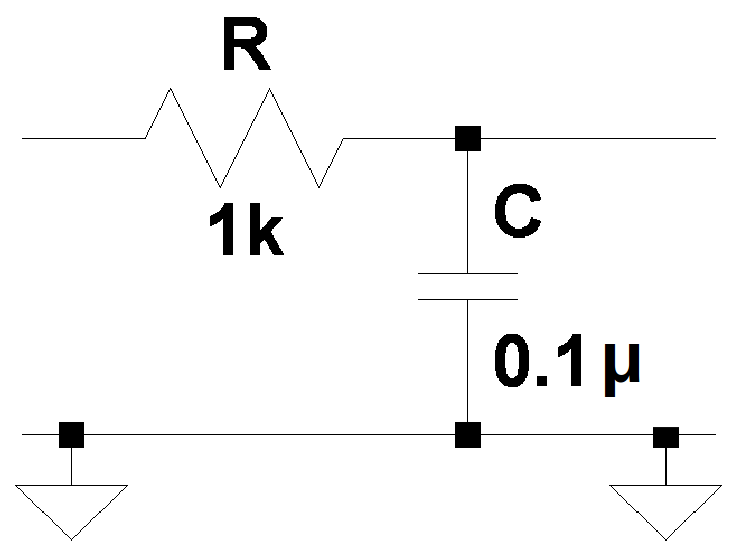
\includegraphics[width=8cm]{LPF.png}
  \caption{測定に用いたLPF}
\end{figure}

この4端子回路の基本行列は、
\begin{equation}
F =
\left[
\begin{array}{rr}
1 & R \\
0 & 1 \\
\end{array}
\right]
\left[
\begin{array}{rr}
1 & 0 \\
sC & 1 \\
\end{array}
\right]
=
\left[
\begin{array}{rr}
1+sRC & R \\
sC & 1 \\
\end{array}
\right]
\end{equation}

伝達関数$\frac{V_{out}\left(s\right)}{V_{in}\left(s\right)}$は、1行1列目の成分の逆数だから、
\begin{equation}
H\left(s\right) = \frac{1}{1+sRC}
\end{equation}
従って、極が実数軸上に一つである。(図)
抵抗値と容量値を代入してその値を求めると、$s = -10^4$である。
\begin{figure}[H]
  \centering
  
\includegraphics[width=5cm]{token.png}
  \caption{周波数特性測定に用いたLPFの入出力電圧比の極}
\end{figure}

周波数は虚軸上正の部分を動くから、
振幅特性は周波数0で最大、周波数が増大するにつれ(2)式の分母が大きくなって減少し、
位相特性は周波数0で0、周波数が増大するにつれ(3)式の第二項が大きくなって減少する。

\subsubsection{HPF}
図5に、測定に用いたRC低域通過フィルタを、素子の値とともに示す。
\begin{figure}[H]
  \centering
  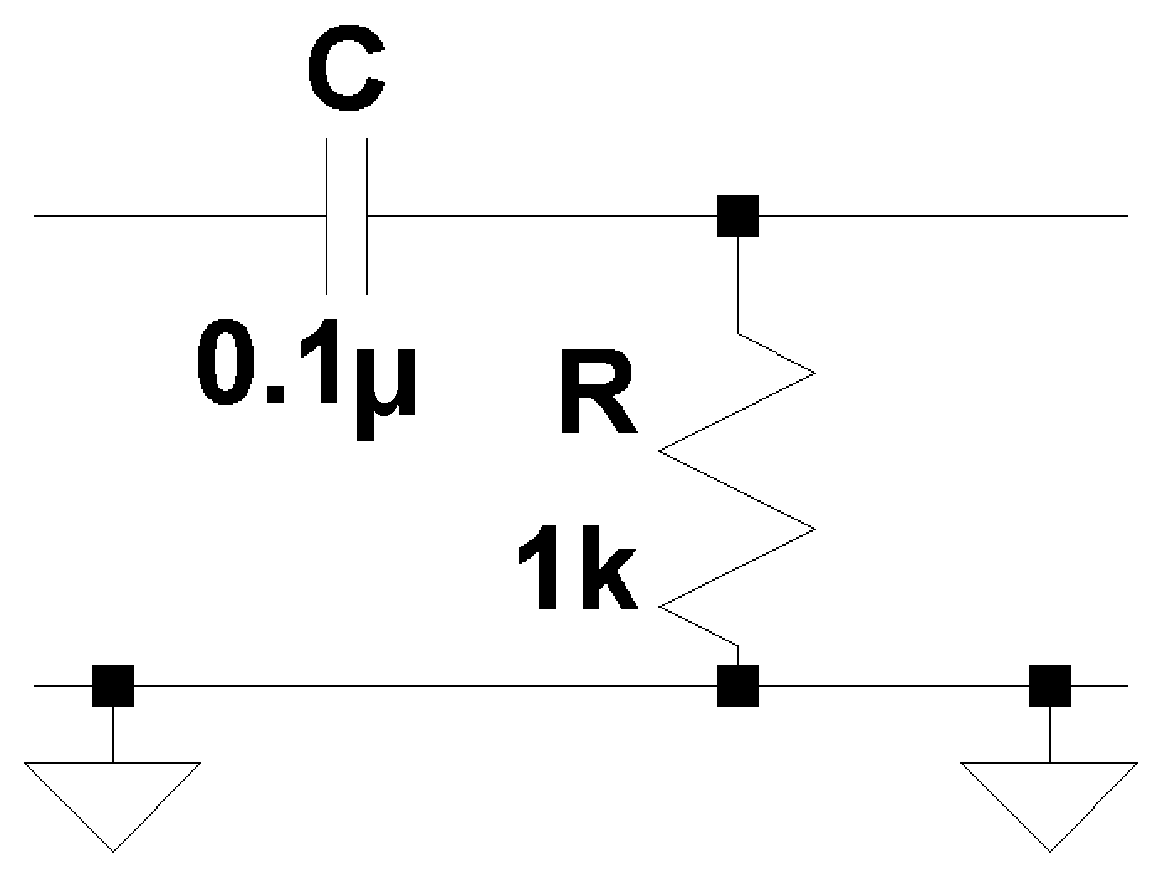
\includegraphics[width=8cm]{HPF.pdf}
  \caption{測定に用いたHPF}
\end{figure}

この4端子回路の基本行列は、
\begin{equation}
F =
\left[
\begin{array}{rr}
1 & \frac{1}{sC} \\
0 & 1 \\
\end{array}
\right]
\left[
\begin{array}{rr}
1 & 0 \\
\frac{1}{R} & 1 \\
\end{array}
\right]
=
\left[
\begin{array}{rr}
1+\frac{1}{sCR} & \frac{1}{sC} \\
\frac{1}{R} & 1 \\
\end{array}
\right]
\end{equation}

LPFと同様に、伝達関数は、
\begin{equation}
H\left(s\right) = \frac{1}{1+\frac{1}{sCR}} = \frac{CR}{CR+\frac{1}{s}}
\end{equation}
従って、極が実数軸上に一つ、原点が零点である。
抵抗値と容量値を代入して極の値を求めると、$s = -10^4$である(図6)。
\begin{figure}[H]
  \centering
  
\includegraphics[width=5cm]{token.png}
  \caption{周波数特性測定に用いたHPFの入出力電圧比の極と零点}
\end{figure}

周波数は虚軸上正の部分を動くから、
振幅特性は周波数0で0、周波数の増大による極との距離と零点との距離の比が1に近づいていく。
位相特性は(3)式の第1項が常に$90^{\circ}$で、周波数が増大するにつれ第2項が0から大きくなって減少する。

\subsubsection{APF}
一次のAPFは伝達関数が
\begin{equation}
H\left(s\right) = H \frac{s-\alpha}{s+\alpha}
\end{equation}
である(図9)から、
虚数軸上を周波数が動くと、
周波数が増大するにつれ、(3)式第1項第2項ともに0で、
周波数が増大するにつれ絶対値を等しくして逆向きに角度を増大させる。
極限では絶対値としては $90^{\circ}$ に収束していくから
全体としては $-180^{\circ}$ に収束する。
\begin{figure}[H]
  \centering
  
\includegraphics[width=5cm]{token.png}
  \caption{周波数特性測定に用いたAPFの伝達関数の極と零点}
\end{figure}

\subsection{インパルス応答を用いた周波数特性の説明}
インパルス応答はステップ応答の時間微分であるから、回路の過渡現象を微分方程式を解析的に解いて求められる。これを周波数領域に変換すると、周波数特性、すなわち伝達関数が得られる。その後は、2.1節と同様に説明できる。

\subsubsection{RLC直列共振回路}
この回路は減衰的なので(2.3節にて詳述)、測定に用いたRLC直列回路のステップ応答w(t)とインパルス応答h(t)は、
\begin{eqnarray}
w(t) &=& \frac{1}{bL} \exp(-at)\sin bt \\
h(t) &=& \frac{\exp(-at)}{bL}\left( -a\sin bt + b\cos bt\right)
\end{eqnarray}
ただし、
\begin{eqnarray}
a &=& \frac{R}{2L} \\
b &=& \left( \frac{1}{LC}-\left(\frac{R}{2L}\right)^2\right)^{\frac{1}{2}}
\end{eqnarray}
$h(t)$をラプラス変換すると、
\begin{equation}
H\left(s\right) = \frac{1}{L}\bullet\frac{s}{\left(s+a\right)^{2}+b^{2}}
\end{equation}
となる。以下は2.1.1節で説明されている。

\subsubsection{RC四端子回路}
測定に用いたRC四端子回路のインパルス応答は、LPF、HPF、APFの順にそれぞれ
\begin{eqnarray}
h_{L}\left(t\right) &=& \frac{1}{RC}\exp(-\frac{t}{RC}) \\
h_{H}\left(t\right) &=& \delta(t) - \frac{1}{RC}\exp(-\frac{t}{RC}) \\
h_{A}\left(t\right) &=& \frac{2}{RC}\exp(-\frac{t}{RC}) - \delta(t)
\end{eqnarray}

で、これらをラプラス変換すると、
\begin{eqnarray}
H\left(s\right) &=& \frac{1}{1+sRC} \\
H\left(s\right) &=& \frac{sRC}{1+sRC} \\
H\left(s\right) &=& \frac{1-sRC}{1+sRC}
\end{eqnarray}
RとCの値を代入すると、$\omega = 10^4$すなわち$f=1.59\si{\kilo\hertz}$が遮断周波数だとわかる。
ここでLPF、HPFの電圧利得が
-3\si{\decibel}
となった周波数と
APFの位相差が $-90^{\circ}$ となった周波数を見てみる
(両対数グラフなので細かい値を読み取ることは困難だが、これらのグラフも図10と図11に示しておく)と、

\begin{description}
 \item[LPF] 1500Hz弱 (1500Hzで-3.10dB)
 \item[HPF] 1700Hz弱 (1700Hzで-2.97dB)
 \item[APF] 1600Hz弱 (1600Hzで$-91.0^{\circ}$)
\end{description}
\begin{figure}[H]
  \centering
  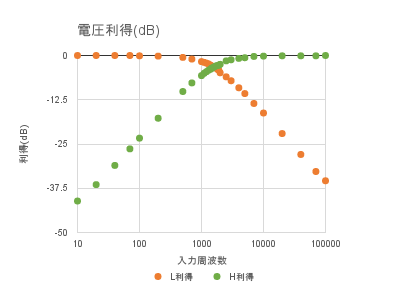
\includegraphics[width=9cm]{ritoku.png}
  \caption{LPFとHPFの電圧利得}
\end{figure}
\begin{figure}[H]
  \centering
  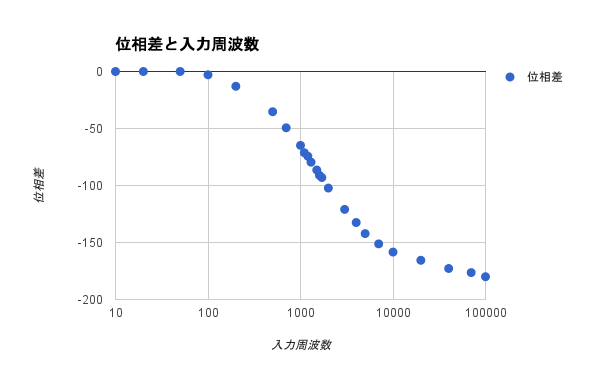
\includegraphics[width=9cm]{isousaApf.png}
  \caption{APFの入出力位相差}
\end{figure}

測定値もあやふやなので正確な誤差率を計算することもかなわないが、十分に理論値に近い値が出ていることがわかる。

\subsection{RLC直列回路のステップ応答}
RLC直列回路のステップ応答は、2.2.1節にて触れた(24)式(ただし、(24)式は入力電圧を1\si{\volt}に固定してしまっている)を含め、以下のごとくである。
\begin{description}
 \item[減衰振動] $w(t) = \frac{V}{bL} \exp(-at)\sin bt$
 \item[臨界減衰] $w(t) = \frac{V}{L} t\exp(-at)$
 \item[過減衰] $w(t) = \frac{V}{cL} \exp(-at)\sinh ct$
\end{description}
ただし、
\begin{equation}
c=\left(\left(\frac{R}{2L}\right)^2-\frac{1}{LC}\right)^{\frac{1}{2}}
\end{equation}
この際、理想的な回路(素子の値も理論値)を考える。周波数測定を行った回路からキャパシタンスとインダクタンスは取り替えず、抵抗だけを直列に増加させていった。

このとき、臨界的である条件は、$R_{all} \simeq 632\si{\ohm}$なので、
まず周波数特性の測定に用いた回路(直列抵抗39.0\si{\ohm})でそのままsテップ応答を観測し、
次に300\si{\ohm}の抵抗を二個、直列に繋ぎたして、
直列抵抗639\si{\ohm}でステップ応答を観測し、
最後に更に1\si{\kilo\ohm}の抵抗を一個、直列に繋ぎたして、
直列抵抗1640\si{\ohm}でステップ応答を観測した。
以下にそのオシロスコープの出力画像(図12、図13、図14)を示す。
\begin{figure}[H]
  \centering
  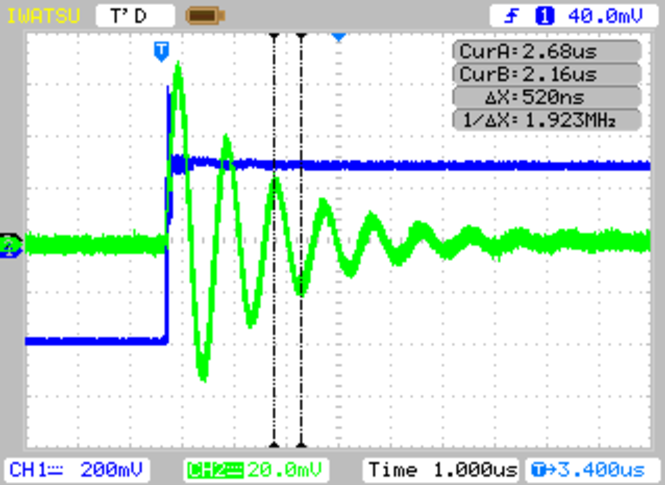
\includegraphics[width=8.5cm]{sindougensui.pdf}
  \caption{RLC回路ステップ応答(直列抵抗39.0\si{\ohm}の場合)}
\end{figure}
\begin{figure}[H]
  \centering
  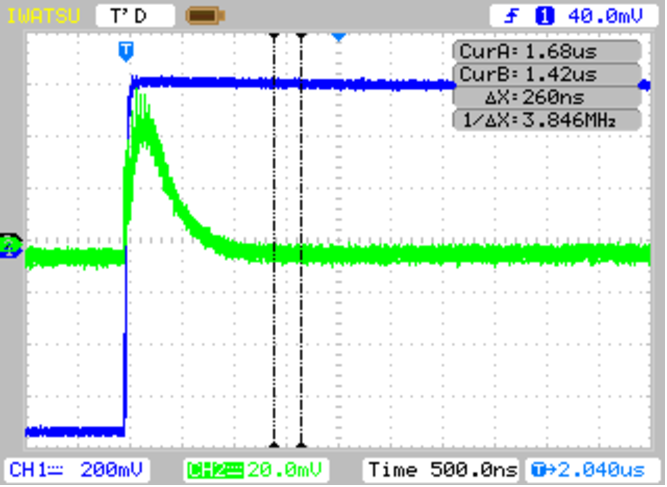
\includegraphics[width=8.5cm]{rinkaigensui.pdf}
  \caption{RLC回路ステップ応答(直列抵抗639\si{\ohm}の場合)}
\end{figure}
\begin{figure}[H]
  \centering
  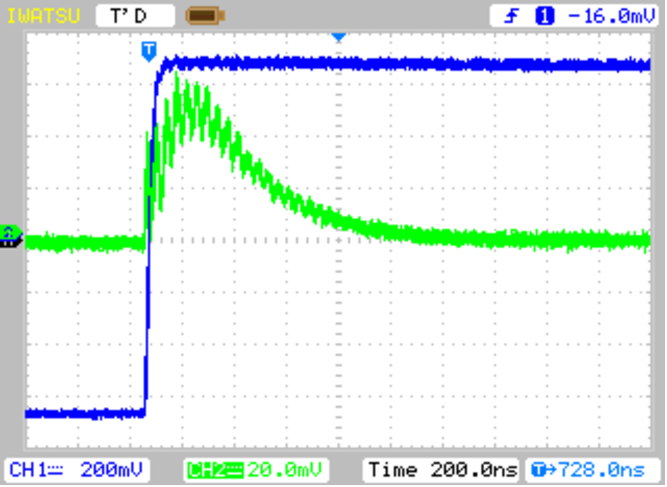
\includegraphics[width=8.5cm]{kagensui.pdf}
  \caption{RLC回路ステップ応答(直列抵抗1640\si{\ohm}の場合)}
\end{figure}

振動減衰の場合について、一つ目のピークの振幅と周期の理論値は
\begin{description}
 \item[一つ目のピークの振幅] 1.95\si{\milli\volt}
 \item[周期] {0.935}\si{\micro\second}
\end{description}
だが、図12を見ると振幅はおおよそ70\si{\milli\volt}を取っている。

臨界減衰の場合について、そのピークの振幅の理論値は1.6\si{\milli\volt}だが、図13を見ると振幅はおおよそ60\si{\milli\volt}である。

過減衰の場合について、そのピークの振幅の理論値は0.9\si{\volt}だが、図14を見ると振幅はおおよそ60\si{\milli\volt}である。

自分の計算が間違っている可能性が高いのだが、
すでにそれぞれ3回計算を繰り返しているので、
どこかで自分が気づけない致命的なミスをしていると考えられる。

\section{付録資料}
これらのプログラムは、実験班員である坂口君が作ったものを目的に合わせて改変して利用したものである。
\lstinputlisting[caption=参考コード1]{P1TFunctionSuikouzumi.py}
\lstinputlisting[caption=参考コード2]{P1analyze.py}

\section{参考資料}
$[1]$ \\
電気電子情報第一(前期)実験テキスト (東京大学工学部電子情報工学科・電気電子工学科)\\
$[2]$ \\
コイルを使う人のための話 (サガミ エレク株式会社 技術統括部) \\
http://www.sagami-elec.co.jp/file/tech/coil\_doc\_100j.pdf \\
$[3]$ \\
電気回路の基礎 (曽根悟・檀良著 朝倉書店 1986年) \\
$[4]$ \\
伝送工学概論 (岩橋榮治著 東海大学出版会 1994年) \\

\end{document}
